\documentclass[12pt]{article}
\usepackage{fullpage}
\usepackage[utf8]{inputenc}
\usepackage{graphicx}
\usepackage{enumitem}
\usepackage{float}
\usepackage{array}
\usepackage{caption}
\usepackage{subcaption}
\usepackage{array} %to place content in one side of cell in table
\usepackage{datetime}
\usepackage{wrapfig}
\usepackage{amsmath} % to be able to create matrices
\usepackage[headsep=0.5cm,headheight=2cm]{geometry}
\usepackage[parfill]{parskip} %remove the indent (tab) at the beginning of new paragraphs
\usepackage{comment}
\geometry{
a4paper,
total={170mm, 240mm}, %130
left=20mm, %40
top=25mm,
}\usepackage{fancyhdr}

\usepackage[comma,numbers,sort&compress]{natbib}
\bibliographystyle{unsrtnat}
\usepackage[pdfstartview=FitH,
            breaklinks=true,
            bookmarksopen=true,
            bookmarksnumbered=true,
            colorlinks=true,
            urlcolor=blue,
            linkcolor=black,
            citecolor=black,
            ]{hyperref}
\usepackage{pbox}
            
\hypersetup{
    colorlinks=true,
    linkcolor=blue,
    filecolor=blue,      
    urlcolor=magenta,
}

%défini la largeur du trait
\pagestyle{fancy}\renewcommand
\headrulewidth{1pt}
%déclaration du contenu de l'entête
\fancyhead[L]{Zahra Farsijani}
\fancyhead[C]{Medchain}
\fancyhead[R]{Project Report}

\begin{document}

\begin{titlepage}
\center

\includegraphics[width=7.2cm]{Images/EPFL_Logo_SVG.png}\vspace{23pt}\\
\textsc{\Large Laboratory For Data Security (LDS)}\\[0.5cm]

\vspace{25pt}
\hrule
\vspace{0.4cm}
{\Large \bfseries MedChain: A Distributed Authorization and Authentication System for Medical Queries }\\[0.5cm] % Title of your document
\normalsize{Master Semester Project Report}
\vspace{0.4cm}
\hrule 
\vspace{1.5cm}
\begin{minipage}{0.5\textwidth}\large
\begin{flushleft}
\emph{Author:}\\
\textbf{Zahra \textsc{Farsijani}}\\
School of Engineering, Electrical Engineering
\end{flushleft}
\end{minipage}
~
\begin{minipage}{0.4\textwidth}
\begin{flushright} \large
\emph{Professor:} \\
\textbf{Jean-Pierre \textsc{Hubaux}}\\
\emph{Supervisors:} \\
\textbf{Juan \textsc{Troncoso-Pastoriza} }\\
\textbf{David \textsc{Froelicher}}\\
\textbf{Mickaël \textsc{Misbach}}

\end{flushright}
\end{minipage}\\
\vfill
\vspace{5pt}
\vspace{20pt}
{\large \today}\\[12cm]
\vfill
% 	\vspace*{\fill}
% 	\begin{center}
% 		\vspace{0.8cm}
% 		{\LARGE Self-sealing icycle innertubes\\
% 		Assessment of design, manufacturing and marketing feasibility \par}
% 		\vspace{0.7cm}		
% 		{\large Fatemeh Farsijani \\ Pavel Kalinin\\ Raúl Núñez \\ Valentin Perruchoud \\ Rachel Wong Min\par}
% 		\vspace{0.7cm}
% 		\today
% 		\\
% % 		\vspace{0.4cm}
% % 		
\includegraphics[width=6.5cm]{Images/EPFL_Logo_SVG.png}
% 	\end{center}
% 	\vspace*{\fill}
\end{titlepage}		
\pagebreak

%\section*{Abstract}
%\addcontentsline{toc}{section}{\protect\numberline{}Abstract}
\newgeometry{left=3cm,right=3cm}
\begin{abstract}

There is great body of research that depends on use and analysis of clinical and health data as well as sharing them among multiple institutions in some way. This gives rise to some concerns and issues regarding the privacy of data. A number of software solutions have been developed in order to address this problem and allow privacy-preserving analysis and sharing of sensitive medical data such as MedCo \cite{raisaro2018medco}, being the very first operational one. However, when it comes to authentication and authorization of data users, MedCo exhibits some limitations. First, in MedCo, both authentication and authorization are central which introduces a single point of failure within the network that can compromise the whole network. Second, each participant in MedCo cluster runs its own access management process. Also, there is no distributed immutable logging of queries received in MedCo. 

In this project, we aim to improve and fully implement ``MedChain: a distributed authorization system for medical queries" that overcomes the drawbacks present in MedCo. MedChain works seamlessly with MedCo and complements its workflow by handling the access management in a distributed manner. MedChain offers auditability as it records all the medical queries from the users in an immutable distributed ledger, i.e., the blockchain.


\end{abstract}
\restoregeometry




\pagebreak

\tableofcontents
\pagebreak

\section{Introduction}\label{section1}
\subsection{Problem Definition and Objectives}

In this project, we aim to implement a distributed authorization system for medical queries, called MedChain that was designed and partly implemented in a previous project. We also intend to make this system specifically compatible with the ecosystem of \href{https://medco.epfl.ch/}{MedCo} and integrate it with it. MedCo is an existing technology that enables privacy-preserving analysis and sharing of medical data. In MedCo, authentication and authorization are centralized; we aim to integrate MedChain into MedCo in order to enable distributed authorization and avoid single point of failure introduced by the centralized system. Furthermore, in MedChain, we introduce distributed immutable logging of system transactions which allows auditability of activities and queries and can thus be used to prevent malicious activity or data misuse. 



% MedCo already has authentication and authorization mechanisms in place, however, they have some drawbacks which Medchain tries to address. First, in the current implementation of MedCo, both authentication and authorization are centralized. This introduces a single point of failure in the whole ecosystem and has to be avoided. Second, hospitals and medical institutions that participate in MedCo cluster have their own identity providers and run access management protocols individually as these processes can not be done in a federated manner. Our proposed software system, Medchain, offers solutions for such shortcomings. It also puts forward other sought-after properties, such as auditability by recording all the queries submitted to it in a blockchain, which is explained in more details later in this report. 

% Some intro and general ideas about the project and how it is relevant to MedCo. Then speaking \textbf{briefly} about what was done last semester and finally the goals and achievements of this semester's project and how it complements the previous work. (Throughout the report, I will make sure that I focus on what has been done this semester, especially, if there are references to work done last semester.)

\subsection{Threat Model}
In this section, we explain the adversaries that we considered during system design and implementation. For every adversary, we consider the scope for their capabilities as well the risks they incur to the system.

MedChain is responsible for distributed authorization of medical queries submitted to MedCo and is thus part of a MedCo network. MedCo network consists of a clinical research network that includes several clinical sites organized in a decentralized federation. Clinical sites provide databases that are maintained and monitored separately. There are also investigators who use MedCo to explore medical data \cite{raisaro2017medco}. Before authenticated investigators can access the data, they need to be \textbf{authorized by MedChain}. Hence, the following adversaries are considered:

\paragraph{Clinical sites:} In general, clinical sites are assumed to provide correct information. However, sites do not necessarily trust each other. 

\paragraph{Regular user/investigator:} This could be a typical user, such as an authorized nurse or physician at a clinical site's research department, who accesses the clinical data and is assumed to be honest-but-curious (HBC) adversary.  

\paragraph{(Tech-savvy) investigators:} This includes authorized investigators as well as black-hat or white-hat hackers who are assumed to be malicious-but-covert (MBC) adversaries as they may try to DOS the system or infer data by performing multiple queries of data. 

\subsection{Requirements}
MedChain should allow distributed authorization of MedCo queries based on defined and agreed multi-signature rules, i.e., authenticated users should be able to query certain sensitive information only after the access management rules have been met. Furthermore, while checking the authorizations of users for their queries, MedChain should keep an immutable and distributed record of all queries submitted to MedCo so that the system can be audited and malicious activities, attacks, or data leakage can be identified and prevented. Last but not least, as part of MedCo ecosystem, MedChain should be able to work seamlessly with all systems that function within MedCo ecosystem, most prominently, \href{https://github.com/ldsec/medco-connector}{MedCo-connector} that orchestrates MedCo queries. 

% \subsection{Report Outline}
% In this report, we first provide some background information on the underlying technologies used in Medchain deployment in Section \ref{section2}. Next, in Section \ref{section3}, design and architecture of Medchain is presented and discussed. In Section \ref{section4}, we give a full descriptions of our solution, its software design and building blocks. Later, in Section \ref{section5}, we discuss the performance of our software solution and its limitations. In Section \ref{section6}, we discuss the future opportunities to improve the solution and, finally, we finish with conclusions in Section \ref{section7}.

% Very brief overview of various sections of the report. (not needed maybe??)

\section{Background}\label{section2}
In this section, we provide some background information about the building blocks of Medchain and some technologies used in its development. 

\subsection{Cothority}\label{cothority}
% A brief overview of Cothority and some of its modules/capabilities that were used. 

As it was mentioned before, MedChain should be able to perform authorization checks in a distributed manner. To achieve this, we used collective authority in MedChain. Collective authority (cothority) available at \cite{cothority:2019} is a project developed and maintained by DEDIS lab at EPFL. Its objective is to provide various frameworks for development, analysis, and deployment of decentralized and distributed (cryptographic) protocols. Servers that provide Cothority framework, services, and protocols are referred to as \textbf{cothority} nodes or \textbf{Conodes} \cite{conode:2019}.  

% We decided to use conodes due to the distributed protocols they offer and thus every Medchain server is a conode. In the following sections, we look at some of the most important building blocks of Cothority as well its services and protocols that play functional role in Medchain. 

 
 \subsubsection{Conode}\label{background:conode}
%  Briefly mention what a conode is and also how it is relevant to MedChain architecture (i.e., a MedChain node is in fact an adapted Conode) with pointers to subsequent sections.

MedChain is a customized Conode capable of performing desirable tasks. This is achieved through definition and implementation of MedChain services and protocols in a general Conode. This is further explained in Section \ref{section3} and Section \ref{section4}.
% As it was mentioned earlier, a \textbf{conode} is a server and conodes are linked together to form a cothority. Clients need to run conodes, either locally for local tests or in public mode in order to access decentralized protocols and services offered by cothority.

% To operate a conode, one needs to correctly set up a host and run the conode program. The reader is referred to conode documentation and instructions on how to setup and use it found at \cite{conode:2019}.


\subsection{ByzCoin}\label{background:byzcoin}
% Briefly explain what is ByzCoin and its various components such as Skipchain, Client transaction, etc. that are relevant to MedChain.  

 ByzCoin \cite{byzcoin:2019} is an open decentralized blockchain system based on Byzantine fault tolerant (BFT) consensus algorithm. The \textbf{Omniledger} paper \cite{kokoris2018omniledger} describes the protocol that ByzCoin implements. ByzCoin uses the Skipchain \cite{skipchain:2019} as its underlying data-structure for storing distributed ledger of keys and values. 

 Skipchain holds the instances of ByzCoin Smart Contracts (we can consider a smart contract as a class and its instance as an object of this class). Actions that affect these instances result in updates in Skipchain. Instances play an important role in MedChain: each of the queries MedChain receives and tries to authorize is an instance of a smart contract defined specifically for MedChain (this is more explained in Section \ref{section3} and Section \ref{section4}). 
 
 In ByzCoin, every instance is stored with the following information in the global state:

\begin{itemize}
    \item \textbf{InstanceID}: It is a globally unique identifier of the instance.
    \item \textbf{Version}: It is the version number of \textit{this} update to the instance, starting from 0.
    \item \textbf{ContractID}: It points to the contract that will be called if the instance receives an instruction to change the instance from the client.
    \item \textbf{Data}: It is the key-value pair that is interpreted by the contract and can change over time.
    \item \textbf{DarcID} It is the ID of the Darc that controls access to the instance. (see below).
\end{itemize}

 
 Below, we explain some important ByzCoin concepts and terminology that are later referred to in this report. 
 
% There are various basic data structures used in ByzCoin. Below, we provide a brief overview of the most relevant ones:
\begin{itemize}
    \item{\textbf{Instructions}}: It is a request to update the ledger and is created by the client. It can be a:
    \begin{itemize}
        \item \texttt{Spawn}: create a new instance
        \item \texttt{Invoke}: call a method of an instance such as \texttt{update}
        \item \texttt{Delete}: remove an instance
    \end{itemize}
    An accepted instruction results in a \texttt{StateChange}. 
    
    \item{\textbf{ClientTransaction}}: A \textit{ClientTransaction} holds a collection of instructions and is sent to conodes in the roster for execution.
    
    \item{\textbf{StateChange}}: The execution of \textit{ClientTransaction}s results in 0 or more changes in the global state referred to as \textit{StateChange}. 
    
    \item{\textbf{Distributed Access Right Controls (Darcs)}}: Darcs define rules to access available resources (such as contract instances) in ByzCoin. Darc plays a pivotal role in MedChain as the main entity that enables authorization. Please refer to Section \ref{background:darc} to learn more about Darcs in MedChain. 

\end{itemize}

% \subsection{} \label{background:smart_contract}

% A somewhat detailed introduction of smart contracts in Cothority
 

% Byzcoin uses coins as the mining reward. At the input a list of all available coins it provided to the contract. After the contract is run, it needs to return the new list of coins that are available. 

% Below, you can find the list of input arguments given to a contract and its output arguments:

% \textbf{Input arguments}: 
% \begin{itemize}
%     \item pointer to database for read-access
%     \item Instructions sent from the client
%     \item key/value pairs of available coins 
% \end{itemize}

% \textbf{Output arguments}: 
% \begin{itemize}
%     \item one StateChange (may be empty)
%     \item updated key/value pairs of remaining coins
%     \item error that will abort the clientTransaction if it is non-zero. If any contract returns non-zero error, the state will not be changed.
% \end{itemize}

% \subsubsection{Contract Instance Structure}

% In ByzCoin, the global state holds the instances of contracts and is split by the Darcs that define the access to control the corresponding instances. Every instruction sent to an instance must resolve the rule in the governing Darc. 



% \subsubsection{Interaction between Instructions and Instances}
% Once a client sends an instruction, he/she indicates the InstanceID to which it corresponds per an instruction argument. ByzCoin tries to first authorize the instruction through the process described in Section \ref{background:darc}, it then uses the \texttt{InstanceID} to look up the responsible contract for the instance and then send the instruction to that contract. 


\subsubsection{Distributed Access Right Controls (Darcs)}\label{background:darc}

% A detailed discussion of a DARC as a pivotal component of MedChain.

In ByzCoin, Darcs are used to manage access to contracts/objects and can thus be used to handle authorizations. Each Darc is a data structure that holds a set of rules as action-expression pairs, i.e., a set of identities (i.e., public keys) in form of an expression is pared with a certain action. Rules must be fulfilled so that the instructions on the instances governed by the Darc can be executed. An example of a Darc action/expression pair is: \texttt{invoke:ContractX.update - "ed25519:<User1's public key> | "ed25519:<user2's public key>"}, which means that either of users 1 or 2 can update the instances of \texttt{ContractX}. Rules defined in Darcs can be \textit{evolved} based on a threshold number of keys. This essentially means that instead of having a static set of rules (e.g., a fixed list of identities that are allowed to access a resource), we can evolve the existing rules any time and thus achieve dynamism in access right definitions.  

% A Darc is a data structure that has a set of rules that define what permissions are granted to any identity (i.e., public key) as pairs of action/expression. . 


Every instruction sent to an instance must resolve the rule in the governing Darc. This means that once a client sends an instruction, he/she indicates the InstanceID to which it corresponds per an instruction argument. ByzCoin tries to first authorize the instruction by considering the relevant rules in the Darc governing the instance. If the rule is fulfilled, ByzCoin uses the \texttt{InstanceID} to look up the responsible contract for the instance and then send the instruction to that contract for execution.



% Every Darc is stored with an \texttt{InstanceID} that is equal to the Darc's \texttt{baseID}. Once a Darc is evolved (i.e., its rules are updated, see later), this \texttt{InstanceID} is overwritten with the new value. Whenever the client sends an instruction for execution, he/she has to also provide the \texttt{InstanceID} of the Darc (i.e., DarcID) that governs the corresponding contract instance, e.g., \texttt{ContractX}, that is to be affected by the instruction. Thus, the Darc comes into play and checks if the client has the right to execute the instruction and consequently, approves or rejects the instruction on the instance. 

The authorization process can be summarized into the steps below:

\begin{enumerate}
    \item Client sends the following instruction to ByzCoin (some fields are omitted for clarity):
    \begin{verbatim}
    InstanceID: <Darc's InstanceID>,
        Invoke:{
            ContractID: ContractX,
            Command:    "update",
            Args:{
                    Name:  query.ID,             
                    Value: []byte(query.Status), 
                },
        }
    \end{verbatim}
    \item ByzCoin finds the Darc instance using the Darc's \texttt{InstanceID} provided by the client in the instruction.
    \item ByzCoin creates an \texttt{Invoke:update} instruction on ContractX's instance to update the key-value pair provided in \texttt{Args}.
    \item ByzCoin checks the Darc found in step 2 and verifies that the request corresponds to the \texttt{invoke:update} rule (i.e., expression) in the Darc instance for the given identity (the client who creates this transaction).
\end{enumerate}

%  A Darc can be updated by an \textit{evolution} process: the identities that have the evolve permission (i.e., \texttt{darc:evolve}) in the Darc create a signature and sign off the new Darc. There is no limit to the number of evolutions that can be performed and evolutions result in a chain of Darcs, also known as a path. A path can be verified by starting at the oldest Darc (also known as the base Darc), walking down the path and verifying the signature at every step. Delegation is also possible in Darcs. That is, a Darc can be given \texttt{evolve} permission to evolve other Darcs and thus evolve the path.

\subsection{MedCo}\label{background:medco}
% A brief introduction of what MedCo is.

MedCo \cite{raisaro2018medco} is a system that enables sensitive medical data to be explored and shared in a  privacy-preserving manner. MedCo guarantees data privacy using collective encryption provided by collective authority \cite{syta2015certificate}. It aims to distribute trust among various medical data providers (such as clinical sites) so that their data can be used and queried by external users while privacy is preserved. 

MedCo is built on top of existing and open-source technologies: (i) i2b2 \cite{murphy2010serving} is a clinical research platforms and together with SHRINE \cite{weber2009shared} they enable clinical data exploration; (ii) UnLynx \cite{froelicher2017unlynx} allows distributed and secure data processing in MedCo. 

In MedCo, user authentication is provided by \href{https://www.keycloak.org/about}{Keycloak} which authenticates users using \href{https://openid.net/connect/}{OpenID Connect} as the identity provider. In the following sections, we will provide more details about how MedChain enables distributed authorization and works with MedCo. 

\section{Design and System Architecture}\label{section3}
\subsection{General Overview} \label{arch:general Overview}
In this section, we look at the architecture of MedChain system. We first begin by considering the requirements that our software solution should be able to fulfil. Then, we discuss how our solution satisfies the requirements and objectives. 

% Full discussion of MedChain architecture design requirements, its final architecture, and the reasoning behind certain choices made in the design. Trying to make it as visual as possible with quality figures. 

% \textbf{Question}: Is it necessary that I contrast the work that has been done last semester and this semester \textit{in this section} as well?? If yes,  any ideas how I can best do that?


\subsection{Requirements} \label{arch:requirements}

The main goal of MedChain is to offer distributed access management mechanisms for MedCo. We started to design and implement MedChain last semester in another project. The main goal of this project is to improve MedChain software already implemented, develop a docker-based implementation of MedChain and integrate MedChain into MedCo described in Section \ref{background:medco}. To achieve this, Medchain has to fulfil the following tasks and requirements:
% \begin{enumerate}
%     \item Offer its services in a distributed manner 
%     \item Offer access management and user authentication 
%     \item Authorize users and queries
%     \item Enable auditability by recording a full history of queries in blockchain
%     \item Work seamlessly with MedCo
% \end{enumerate}
% In the following sections, we study how each of the above-mentioned requirements are fulfilled in Medchain. 

% \subsubsection{Distributed Services in Medchain} \label{arch:distributed}
% As it was mentioned in the previous section, the first goal of Medchain is to offer services in a distributed manner. To achieve this, we used conodes. Conodes make the foundation for Medchain. They support distributed protocols and services provided by the \href{https://github.com/dedis/onet/blob/master/README.md}{onet} library (a part of Cothority project developed by DEDIS at EPFL). Consequently, Medchain is able to offer access management in a distributed manner. 

% \subsubsection{Authentication in Medchain}\label{arch:authentication}
% The goal of authentication is to verify the identity of the user who wants to access a specific resource such as data. In Medchain, user authentication is delegated to Keycloak \cite{keycloak:2019} which is the identity provider. This means that once Medchain receives a query from a user, we can simply assume that he/she is already authenticated and his/her identity and the user identity is submitted to Medchain as part of the query. We will discuss this in more details in Section \ref{arch:flow}, where the flow of query in Medchain is described comprehensively.

\subsubsection{Authorization in Medchain}\label{arch:authorization}
The goal of authorization is to control the user access to resources (e.g., sensitive medical data) based on agreed rules. In MedChain, we use Darcs (described in Section \ref{background:darc}) to enable user authorization and access management. 


\subsubsection{Distributed Immutable Logging in MedChain} \label{arch:audit}
% Auditability in Medchain means that there should be a mechanism in place so that the users can track all the queries submitted to Medchain server. Consequently, trace of any data misuse, data abuse, security/privacy breach, etc. can be found and mitigated later. 

In MedChain, we use blockchains to offer distributed auditability. The blockchain framework we use in MedChain is ByzCoin (see Section \ref{background:byzcoin}). Every query sent to MedCo by the user as well as its status, whether it is authorized or rejected, is recorded in the immutable ledger that is accessible at every MedChain node in the network.  

\subsection{Medchain High-level View} \label{arch:high-level view}

Figure \ref{fig:medchain_node} shows how a MedChain node looks like. Every MedChain node is a customized Conode (see section \ref{section4} for further details) and has one or more projects defined in it. Projects specify user access controls and define data resources. Each project contains three important building blocks. Below you can find more about projects and their building blocks:
\begin{itemize}
    \item \textbf{Projects}: specify rules for users to access data resources using access right controls.
    \item \textbf{Smart contracts}: define data, in this case key-value pairs of the query (i.e., the key) and its status (i.e., the value), that is stored in distributed ledger
    \item \textbf{Darcs}: define and manage user's access to resources. Every project is attached to a single Darc that determines user access rules for the database governed by the project. 
    \item \textbf{Blockchain}: system audit. It is possible to retrieve a record of all queries submitted to MedChain for authorization to check the content of query and the querier's identity. 
\end{itemize}


\begin{figure}[ht] 
        \centering 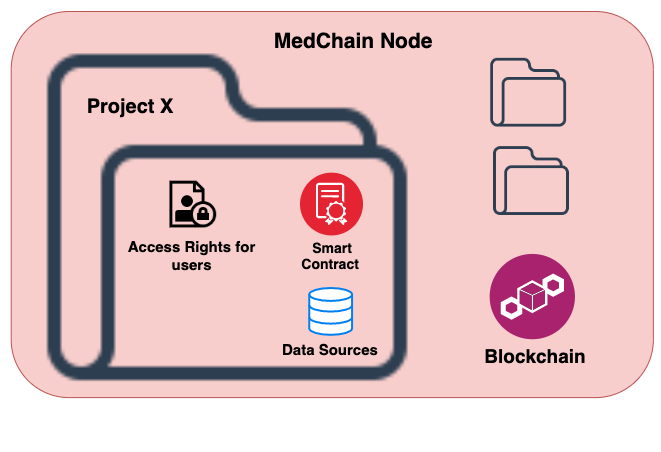
\includegraphics[width=0.7\columnwidth]{Images/medchain_node.png}
        \caption{\label{fig:medchain_node} 
         The structure and building blocks of a MedChain node.
        }
\end{figure}




\subsection{Flow of Queries in Medchain}\label{arch:flow}

Figure \ref{fig:medchain_workflow} illustrates the full architecture of MedChain and its detailed workflow starting from query creation and submission by the client until the query is executed. The numbers used in the figure correspond to the steps described below. Also, parts outlined with dashed-line represent the contributions done in this project (further explained in Sections \ref{section4}, \ref{section5}, and \ref{section6}).

% In this figure, there are three hospitals each running their own local Medchain server (conode). Now, focusing only on the user at Hospital 1, we describe the enumerated steps in Figure \ref{fig:medchain_workflow} as following:

\begin{enumerate}
    \item \textbf{User Login}: Client receives the token (i.e., its identity) from Keycloak (using OpenID Connect).
    
    \item \textbf{Query Creation \& Submission}: User spawns a query. The query is submitted to MedCo-connector (i.e., query orchestrator). Figure \ref{fig:medco_query} shows the simplified structure of a MedCo-connector (explore) query. 
  \begin{figure}[htbp] 
        \centering 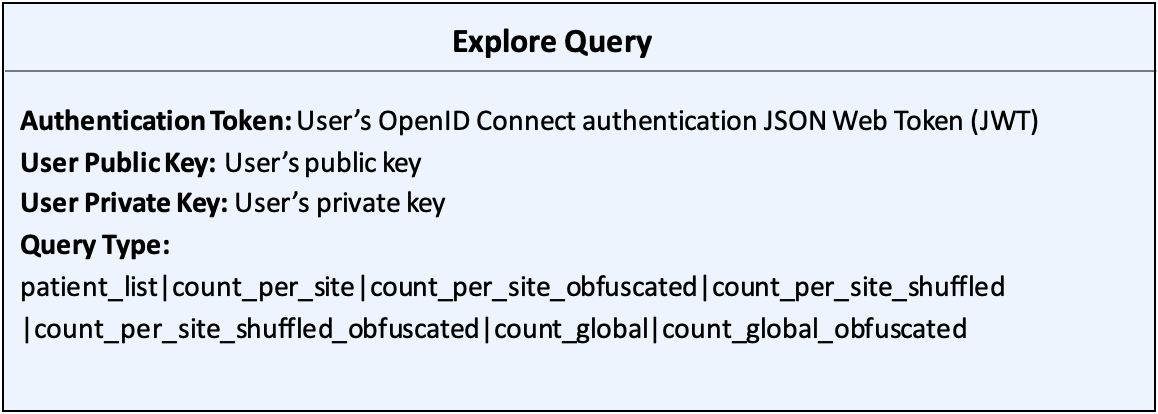
\includegraphics[width=0.9\columnwidth]{Images/medco_query.png}
        \caption{\label{fig:medco_query} 
         Simplified structure of a MedCo-connector (explore) query.
        }
\end{figure}
    
    \item \textbf{User Authentication}: MedCo-connector verifies the token (i.e., the identity) of the user and authenticates it. 
    
    \item \textbf{Submission of Query To Medchain}: MedCo-connector receives the user identity and user query. It then sends the query that contains the user’s identity (i.e., part of the token) to MedChain server for authorization. The query that MedChain receives is a key-value pair data structure shown in Figure \ref{fig:medchain_query}:
\begin{figure}[htbp] 
        \centering 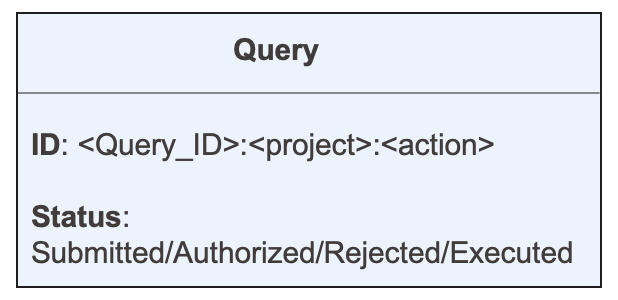
\includegraphics[width=0.5\columnwidth]{Images/query.png}
        \caption{\label{fig:medchain_query} 
         MedChain query data structure
        }
\end{figure}

%     \begin{verbatim}
%         {ID:<Query ID>,Status:<Query Status>}
%     \end{verbatim}
% The query itself has the following format:
%   \begin{verbatim}
%       <user_id>:<databaseX>:<type of query>
%   \end{verbatim}
  Where \texttt{<Query\_id>} contains part of the user's token provided by Keycloak, \texttt{<project>} is the name of the project (i.e., the database) the user is querying, and \texttt{<action>} is what the user is trying to access from the database which can be one of the below:
  \begin{itemize}
        \item \texttt{patient\_list}
        \item \texttt{count\_per\_site}
        \item \texttt{count\_per\_site\_obfuscated}
        \item \texttt{count\_per\_site\_shuffled}
        \item \texttt{count\_per\_site\_shuffled\_obfuscated}
        \item \texttt{count\_global}
        \item \texttt{count\_global\_obfuscated}
  \end{itemize}
   
  Finally, \texttt{Status} is the status of the query in MedChain and it could be: \texttt{"Submitted"}, \texttt{"Authorized"}, \texttt{"Rejected"}, or \texttt{"Executed"} .

    \item \textbf{Query Transaction Creation}: \label{workflow:step 5}
    MedChain retrieves the ID o the Darc based on the name of the project and creates a normal (i.e., not deferred, see later) transaction to spawn a \texttt{Query} (i.e., an instance of \texttt{MedChain Contract}) and signs it. The transaction looks like below:
        \begin{verbatim}
CreateTransaction(byzcoin.Instruction{
    InstanceID:    byzcoin.NewInstanceID(<Project X Darc ID>),
    Spawn: &byzcoin.Spawn{
        ContractID: MedChainContractID,
        Args: byzcoin.Arguments{
                {
                    Name:  <Query_id>:<projectX>:<action>,
                    Value: []byte("Submitted"),
                },
        },
})
        \end{verbatim}
        
    \item \textbf{Query Authorization}: MedChain retrieves the Darc governing the instance and checks the user authorizations for the \texttt{<action>}. Depending on the result of authorization checks one of the below scenarios happens:
    \begin{itemize}
        \item If the Darc rules \textbf{are not met} (i.e., user is not allowed to query \texttt{<action>}), the query is immediately rejected. Consequently, a new transaction is created by MedChain that \textit{updates} query \texttt{Status} to \texttt{Rejected} and adds the transaction to the ledger. Also, a message containing the new query status is sent back to MedCo-connector in order to notify it of authorization rejection (this is more explained in Section \ref{section4} where MedChain API calls are described)
        
        \item If the Darc rules \textbf{are met}, the query is authorized. Hence, two new transactions are created by MedChain. The first one is a normal transaction that updates the query \texttt{Status} to \texttt{Authorized} which is only signed by this MedChain node and is immediately written to the ledger. The second transaction, however, is a \textit{deferred} transaction (see Section \ref{section4}). By spawning a deferred transaction, MedChain node proposes a transaction to the whole MedChain network i.e., it broadcasts the instance ID of deferred transaction to rest of the MedChain nodes in network. Then, users at other MedChain nodes need to \textit{sign} the transaction using the instance ID they receive. When the rules of Darc are met (i.e., a threshold number of signatures are added to the proposed transaction), the transaction can be executed by any of the signers (only one execution is allowed for every proposed transaction). It is important to note that even if all users can sign the transaction, it can only be executed once the rules of corresponding Darc are met. 
        Once the proposed transaction is successfully executed, the transaction is added to the ledger and MedChain sends MedCo-connector a message containing the status of query as \texttt{Authorized}.  
    \end{itemize}
     
    \item \textbf{Query Authorization Result}: In the mean time, MedCo-connector is waiting for a reply from MedChain node. Once authorization (step 6) is done, MedChain sends the result (i.e., query status) back to MedCo-connector which is either \texttt{Authorized} or \texttt{Rejected}. 
    
    \item \textbf{Query Execution and Committing Final Query Status To The Ledger}: If MedCo-connector learns that the query has been rejected through a message from MedChain node, it will not execute the query. Otherwise, MedCo-connector executes the query and once done, sends a message back to MedChain so that the status of query is updated to \texttt{Executed} and is written to the ledger.

\end{enumerate}
 
 
 The explained workflow and its mechanisms such as MedChain to MedChain communications (i.e., message propagation among MedChain nodes) and API calls have been fully implemented in this project. 
 
 \begin{figure}[htbp] 
        \centering 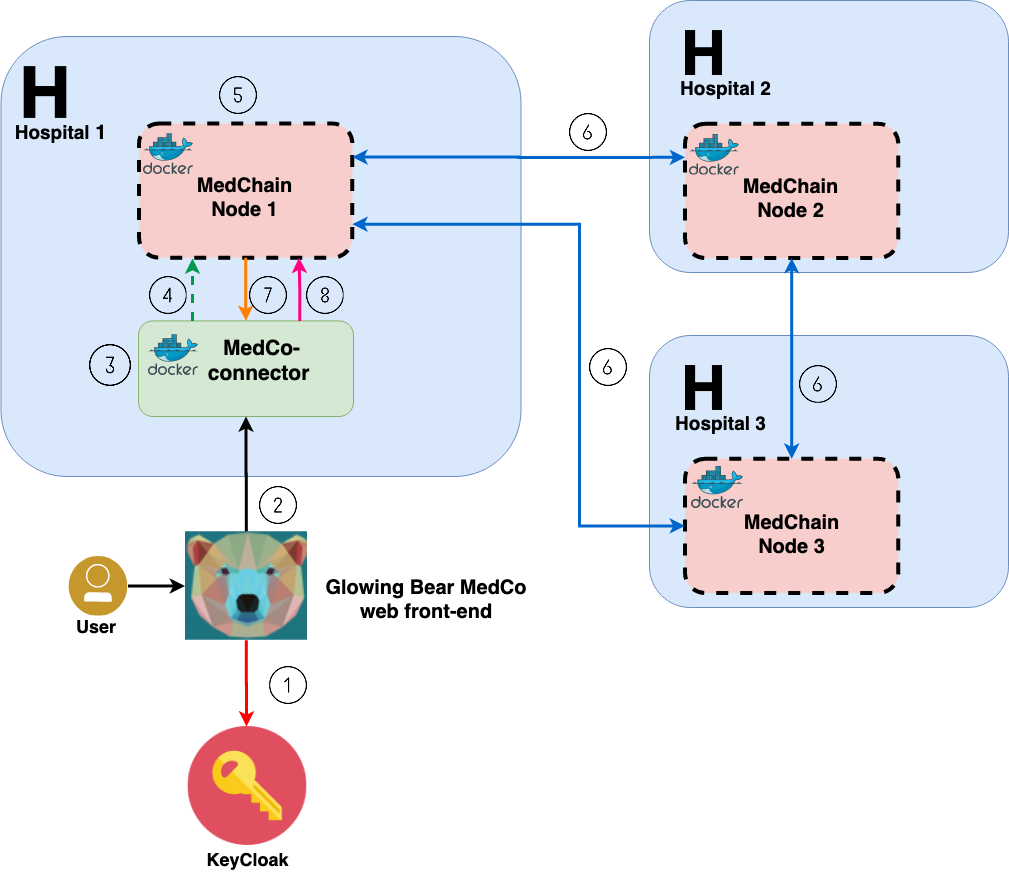
\includegraphics[width=1\columnwidth]{Images/arch-updated.png}
        \caption{\label{fig:medchain_workflow} 
         Medchain architecture: workflow of queries in MedChain.
        }
\end{figure}


\section{System Implementation}\label{section4}
The full Medchain code, it documentation as well as instructions on how to run it is available in \href{https://github.com/ldsec/medchain/tree/dev}{Medchain Github repository}. In this section, we aim to provide details about the code structure of the Medchain and not instructions on how to use the code.  

\subsection{Conode}
Every Medchain node is a cothority server, known as a conode. There are several ways to initialize a conode that are described in conode documentation found at \cite{conode:2019}. In this project, we used \href{https://github.com/dedis/cothority/blob/master/conode/README.md#option-1-computer-configuration-setup-with-the-command-line}{configuration setup with the command line} to setup our network of 3 local conodes in an interactive manner. Also, in order to use the conodes we followed the instructions to \href{https://github.com/dedis/cothority/blob/master/conode/README.md#option-1-computer-run-with-the-command-line}{run} them. 

The main point to note here is that once a smart contract is developed and imported into a conode, it is available and can be used by the client. This means that the user does not need to bootstrap the smart contract or install it.  

\subsection{API}
In this section, we provide details about some building blocks of the Medchain Application Programming Interface (API). 

\subsubsection{Smart Contract} \label{impl:smart_contract}
The smart contract provides the user with the API to interact with the skipchain (i.e., the ledger) by adding, updating, or removing the instances of the contract from the ledger. 

We developed the smart contract in Go using the template contract provided in cothority\_template repository called  \href{https://github.com/dedis/cothority_template/tree/master/byzcoin}{ByzCoin example} which is a simple key-value contract, meaning that every instance of the contract that is recorded in the ledger is a key-value store data structure. Medchain smart contract is identified by its name "\textbf{queryContract}". This contract is distinguishable from any other contract used in Medchain deployment such as Darc contracts (see Section \ref{impl:darcs}). The client uses this ID in order to define which contract instance he/she wants to manipulate. The queries submitted to Medchain are recorded in the ledger as instances of \texttt{queryContract}. The structure of these queries is shown below: 

\begin{verbatim}
type Query struct {
	    ID     string //<query_id>:<user_id:databaseX>:<type of query>
	    Status string // "Submitted", "Authorized", or "Rejected"
} 
\end{verbatim}

As it is shown above, the key of a queryContract instance is the ID of the query and the value is its status.  

To serve the purposes of Medchain, we changed some functionalities of the template contract so that it is adapted to Medchain ecosystem. In ByzCoin, the smart contract has to implement three API methods: \texttt{Spawn},\texttt{Invoke}, and \texttt{Delete}. The very first instance of a contract is created by creating a transaction using \texttt{Spawn} as the instruction. By this transaction, the user sets the query ID as the key of the instance and its status as the value. Later, the user can manipulate this instance of the contract by calling an \texttt{Invoke} on it. The \texttt{Invoke} method in \texttt{queryContract} implements two methods itself: \texttt{update} and \texttt{verifystatus}. Using update, the user is able to retrieve a specific contract instance (i.e., query) from the skipchain by its key (i.e., query ID) and update its value (i.e., the status of the query) if it already exists in the skipchain, however, if that is not the case, a new instance of the contract will be spawned using the provided key-value pair. \texttt{verifystatus} method is used by Medchain server itself to retrieve a query from the ledger and verify its status in a similar manner to \texttt{update} method. In Medchain, we decided not to implement the \texttt{Delete} function in contract as we do not want the user to be able to remove a query (i.e., an instance of the contract) from the global state. 

Whenever a contract instance is created (spawned) it is allocated an \texttt{InstanceID} that is based on the ID of the Darc contract governing it (please refer to Section \ref{background:smart_contract} for more details). Later, this instance of the contract is retrievable and authorized by the Darc controlling it using this \texttt{InstanceID}. 

\subsubsection{Deferred Transactions} \label{impl:deferred_tx}
In a real world scenario, it is not always possible for hospitals (running Medchain servers) to approve queries they receive from other Medchain servers instantly, for example, the hospital manager may not be present or the local Medchain server may be down. Thus, the query will be rejected as it will not receive the threshold number of signatures from other Medchain servers in the network it needs so that it is deemed as approved at the time it is created. There should be a mechanism in Medchain to handle this issue. \textbf{Deferred transactions} can be used as a solution for this problem. As the name suggests, deferred transactions allow a transaction to remain idle until it receives the threshold number of signatures it needs to be written in the ledger.  

In order to enable deferred transactions in ByzCoin server, the developer should define a special method in the smart contract, namely, \texttt{VerifyDeferredInstruction}, which is not implemented in a \texttt{BasicContract} (i.e., the basic data structure that all contracts implement by default). In other words, types which embed \texttt{BasicContract} must override this method if they want to support deferred transactions (using the \texttt{Deferred contract}). 

To enable deferred execution of a \texttt{queryContract} instance, the following steps are taken:
\begin{enumerate}
    \item User spawns a \texttt{queryContract} instance (This is the proposed transaction).
    \item User spawns a \texttt{deferred\_contract} instance with query instance as its arguments.
    \item Signers sign the proposed transaction and invoke an \texttt{addProof} on it.
    \item User invokes an \texttt{execProposedTx} on proposed transaction to execute it.
\end{enumerate}

\subsubsection{Darcs} \label{impl:darcs}
In ByzCoin, Darcs are used to enable authorization and access management and are, in fact, smart contracts. The only difference between a Darc and a general smart contract is that a Darc supports \texttt{actions} and \texttt{expressions} that are used to define a set of rules in a Darc.

ByzCoin offers some Darcs in its \texttt{darc} library such as \texttt{SecureDarc}, however, the developer can also develop his/her own Darc contract. In Medchain, we use \texttt{SecureContract} and have customized it to meet the requirements of Medchain. 

\texttt{SecureDarc} contract defines access rules for all clients using the Darc data structure. Upon starting a cluster of Medchain servers, a new ByzCoin blockchain and a \texttt{genesis Darc} instance are created. The \texttt{genesis Darc} indicates what instructions need which signatures to be accepted. Below, you can see how the \texttt{genesis Darc} we use in Medchain looks like:

\begin{verbatim}

- Darc:
    -- Description: "genesis darc"
    -- BaseID: darc:<ID_genesis_darc>
    -- PrevID: darc:<ID_darc>
    -- Version: 0
    -- Rules:
        --- invoke:config.update_config - "ed25519:<ID_client>"
        --- spawn:darc - "ed25519:<ID_client>"
        --- invoke:darc.evolve - "ed25519:<ID_client>"
        --- invoke:darc.evolve_unrestricted - "ed25519:<ID_client>"
        --- _sign - "ed25519:3<ID_client>"
        --- spawn:naming - "ed25519:<ID_client>"
        --- spawn:queryContract - "ed25519:<ID_client>"
        --- invoke:queryContract.update - "ed25519:<ID_client>"
        --- invoke:queryContract.verifystatus - "ed25519:<ID_client>"
        --- _name:queryContract - "ed25519:<ID_client>"
        --- invoke:config.view_change - "ed25519:<ID_server> 
            | ed25519:<ID_server> | ed25519:<ID_server>"
    -- Signatures:
    
\end{verbatim}

In the above \texttt{genesis Darc}, we can see the pairs of \texttt{action/expression} that define different rules. For example, \texttt{spawn:queryContract - "ed25519:<ID\_client>"} where \texttt{ID\_client} refers to the ID of the client who is granted the permission for the action \texttt{spawn:queryContract}. Darc expressions are a simple language for defining complex policies. For example, in the rule \texttt{invoke:config.view\_change - "ed25519:<ID\_server> | ed25519:<ID\_server>"}, an "\texttt{or}" expression has been used among the IDs of Medchain cluster servers. 

Now, we create Darcs for different projects (e.g., \texttt{Project A} and \texttt{Prject B}) in Medchain. We assume that each project has 3 clients (i.e., one client per Medchain server). We create new Darcs and define rules (i.e., action/expression pairs) for them. As an example, the Darc for project A is given below:

\begin{verbatim}
- Darc:
    -- Description: "Project A Darc"
    -- BaseID: darc:<ID_darcA>
    -- PrevID: darc:<ID_genesis_darc>
    -- Version: 0
    -- Rules:
        --- _evolve - "ed25519:<ID_owner>" 
        --- _sign - "ed25519:<ID_client1>" | 
        "ed25519:<ID_client2>" | "ed25519:<ID_client3>"
        --- spawn:queryContract - "ed25519:<ID_client1>" | 
        "ed25519:<ID_client2>" | "ed25519:<ID_client3>"
        --- invoke:queryContract.update - 
        "ed25519:<ID_client1>" | "ed25519:<ID_client2>" |
        "ed25519:<ID_client3>"
        --- invoke:queryContract.patient_list - 
        "ed25519:<ID_client1>" | "ed25519:<ID_client2>" |
        "ed25519:<ID_client3>"
        --- invoke:queryContract.count_per_site - 
        "ed25519:<ID_client1>" | "ed25519:<ID_client2>" 
        | "ed25519:<ID_client3>"
        --- invoke:queryContract.count_per_site_obfuscated - 
        "ed25519:<ID_client1>" | "ed25519:<ID_client2>" | 
        "ed25519:<ID_client3>"
        --- invoke:queryContract.count_per_site_shuffled - 
        "ed25519:<ID_client1>" | "ed25519:<ID_client2>" |
        "ed25519:<ID_client3>"
        --- invoke:queryContract.count_per_site_shuffled_obfuscated - 
        "ed25519:<ID_client1>" 
        --- invoke:queryContract.count_global - 
        "ed25519:<ID_client1>" 
        --- invoke:queryContract.count_global_obfuscated - 
        "ed25519:<ID_client1>" 
    -- Signatures:
\end{verbatim}

In the above Darc for Project A, we have defined rules using different types of actions and expressions. For example, all users can take action  \texttt{invoke:queryContract.patient\_list} and in order for it to be approved, the signature of \textbf{any} of the signers is enough as an \texttt{OR} expression is used among signers. However, only client 1 is given permission to query \texttt{count\_global} from database A (i.e., the action \texttt{invoke:queryContract.count\_global}). 

Now, let's see how the Darc for Project A can authorize an action. The first step is that the client sends a spawn instruction to Project A Darc contract. Then, the client asks the instance to create a new instance with the \texttt{contractID} of Medchain smart contract, i.e., \texttt{queryContract}, which is different from the ID of the Darc instance itself. The client must be able to authenticate against a \texttt{spawn:queryContract} rule defined in the Project A Darc instance which is indeed the case according to Project A Darc definition above. The transaction that client creates looks like below:

\begin{verbatim}
instr := byzcoin.Instruction{
    InstanceID: byzcoin.NewInstanceID(<Project A Darc ID>),
    Spawn: &byzcoin.Spawn{
    ContractID: "queryContract",
    Args: byzcoin.Arguments{
		    {
		        Name:  < query ID including the action>,
		        Value: []byte("Submitted"), 
		    },
        }  
    },
    SignerCounter: c.nextCtrs(),
}
\end{verbatim}

The new instance spawned will have an instance ID equal to the hash of the Spawn instruction. The client can remember this instance ID in order to invoke methods on it later. In Medchain, we also use \texttt{contract\_name} of ByzCoin. This contract is a singleton contract that is always created in the genesis block. One can only invoke the naming contract to relate a Darc ID and name tuple to another instance ID. Using this contract, the client does not need to store instance IDs as long as they are named and thus, makes it easier for the client to use the instance IDs of the contracts.

After this step, a \texttt{queryContract} instance spawned by the user (which is in fact the query submitted to Medchain from MedCo) is bound to Project A Darc and is governed by it; thus, the Darc can check for the authorizations of the action the client is trying to take. 

\subsubsection{Client Implementation} \label{impl:client}
To implement a client that can interact with Medchain, we used the default clients  implemented in ByzCoin Client library. The \texttt{Client} is a structure that communicates with the ByzCoin service and interacts with it. 

\subsubsection{Services} \label{impl:services}
In Cothority, a Service is a long term entity that is created when a conode is created. It serves different purposes:
\begin{itemize}
    \item serve the client requests
    \item create and launch protocols in the Overlay network
    \item broadcast to and receive information from services on other conodes within the cothority network. 
\end{itemize}

In Medchain, we mainly used two services: ByzCoin and Onet service. These services handle client-server communications and enable the user to interact with the conodes. We define Medchain API using these services and later implement the CLI-program on top of this API (see Section \ref{impl:cli}). Table \ref{tbl:med_api_calls} shows some of the most important API calls defined in Medchain as well as resources they take and their responses.

\begin{table}[ht]
\centering
\caption{Some of Medchain API calls}
\label{tbl:med_api_calls}
\begin{tabular}{|l|l|l|l|}
\hline
\textbf{Name of Method} & \textbf{Description} & \textbf{Resources} & \textbf{Response}\\
\hline
\textbf{CreateQueryAndWait}    &  Spawn a query & \pbox{20cm}{ User ID, \\ Query definition, \\ Query ID }  & OK?\\
\hline
\textbf{UpdateQueryStatus} & Update the status of a query & Query ID  &  OK? \\
\hline
\textbf{VerifyQueryStatus} & Verify the status of a query & Query ID  &  OK? \\
\hline
 
\end{tabular}
\end{table}

To be able to use the services, we need to register them with the default \href{https://github.com/dedis/cothority/blob/master/suite.go}{Cothority suite}. We use the services to define the API and interact with conodes and contracts.


\subsection{App and Command-Line Interface (CLI)}\label{impl:cli}
An application, in the context of Onet, is a CLI-program that interacts with one or more conodes through the use of the API defined by one or more services. 

We implemented the CLI for Medchain using \href{https://github.com/dedis/cothority/tree/master/byzcoin/bcadmin}{bcadmin} library. The CLI allows the user to start a new ByzCoin blockchain, register new users, initialize and manage pre-developed Darcs, interact with the smart contract, etc. through the command-line. The code for this CLI-app is found in \texttt{mc/} directory of Medchain repository. 

%\subsection{Docker-based Implementation}\label{impl:docker}
%TODO

\section{System Evaluation}\label{section5}
%\subsection{Fulfilment of Requirements}

\subsection{Limitations}
Medchain has some limitations in its current version. First, it is the low latency in authorizing queries which results in low query throughput. The latency stems from the fact that for query authorization the \texttt{InstanceID} of the query should be retrieved so that the authorization is based on the responsible Darc that governs the query. Every time a query is spawned, its \texttt{InstanceID} is named so that it is easily fetched from the global state by its name later using function \texttt{ResolveInstanceID()} of ByzCoin. However, this function returns the results very slowly and thus impedes the authorization of other queries in the pipeline. 
Our workaround to overcome this issue was to save the \texttt{InstanceID} of all queries in a secondary data type called \texttt{QueryKey[]} as soon as they are spawned and every time retrieve the \texttt{InstanceID} from \texttt{QueryKey[]} instead of the global state. This method helps improve the speed and remove the overhead of transactions needed for naming the query instances at the price of more space complexity. The other drawback of this workaround is that it is prone to error and cannot be trusted. 

Second, Medchain CLI requires the admin to define project Darcs by adding rules to them at system startup which is both an involved and time-consuming process. We aim to introduce ways to automate this process and make it more straight-forward.  



\section{Future Work}\label{section6}
In this section, we would like to offer some opportunities for further improving our implemented software solution and the results of this project. 

\subsection{Integration with MedCo}
One of the main purposes and requirements of Medchain is to make it work seamlessly with data service providers, specifically MedCo. However, given that this requirement was not fulfilled in the scope of this project, the full integration of Medchain into MedCo is expected to be done in future versions of Medchain.  

\subsection{Use of Deferred Transactions}
Although we were able to implement deferred transactions in Medchain, we have not been able to test their functionality in this project and we are not sure if they function properly as we have only tested this functionality locally. Therefore, it is expected that in the future this functionality will be tested in a multi-node setup and debugged if necessary. 
%\subsection{Improvements}

\section{Conclusion}\label{section7}
In this project, we designed and implemented a distributed authorization and access management system for medical queries called Medchain. Medchain is written in Go and is based on an existing distributed framework called Cothority and runs on conodes. It enables distributed access management through the use of smart contracts (Darcs) and offers auditability through the use of permissioned blockchains for recording all the queries it receives over its lifetime. Medchain is mainly designed to work seamlessly with MedCo and overcome MedCo's authorization limitations.

Medchain supports a CLI interface that enables the user to interact with the cluster of servers through the command-line. In future versions of Medchain, we aim to integrate it with MedCo ecosystem and have it work as part of the whole MedCo workflow. We will also improve its front-end and the user interface.    




%\newpage

%\section{Appendix}\label{section11}
%\input{11Appendix.tex}


\pagebreak
%%%%%%%%%%%%%%%% Bibliography %%%%%%%%%%%%%%%%
\addtocontents{toc}{\vspace{.5\baselineskip}}
\addcontentsline{toc}{section}{\protect\numberline{}{References}}
\bibliography{bibliography}

\end{document}